\chapter{Nodejs and MongoDB CRUD Application}
%Intro\footnotemark\\
\par In this Chapter we will go over the Implementation of an application with Node.js and MongoDB and
carrying out CRUD operations.
\begin{spacing}{1.2}
%note en bas de page
\section{Nodejs installation }
\par Installing npm on our VM.
\\
\begin{figure}[!htb] 
\begin{center} 
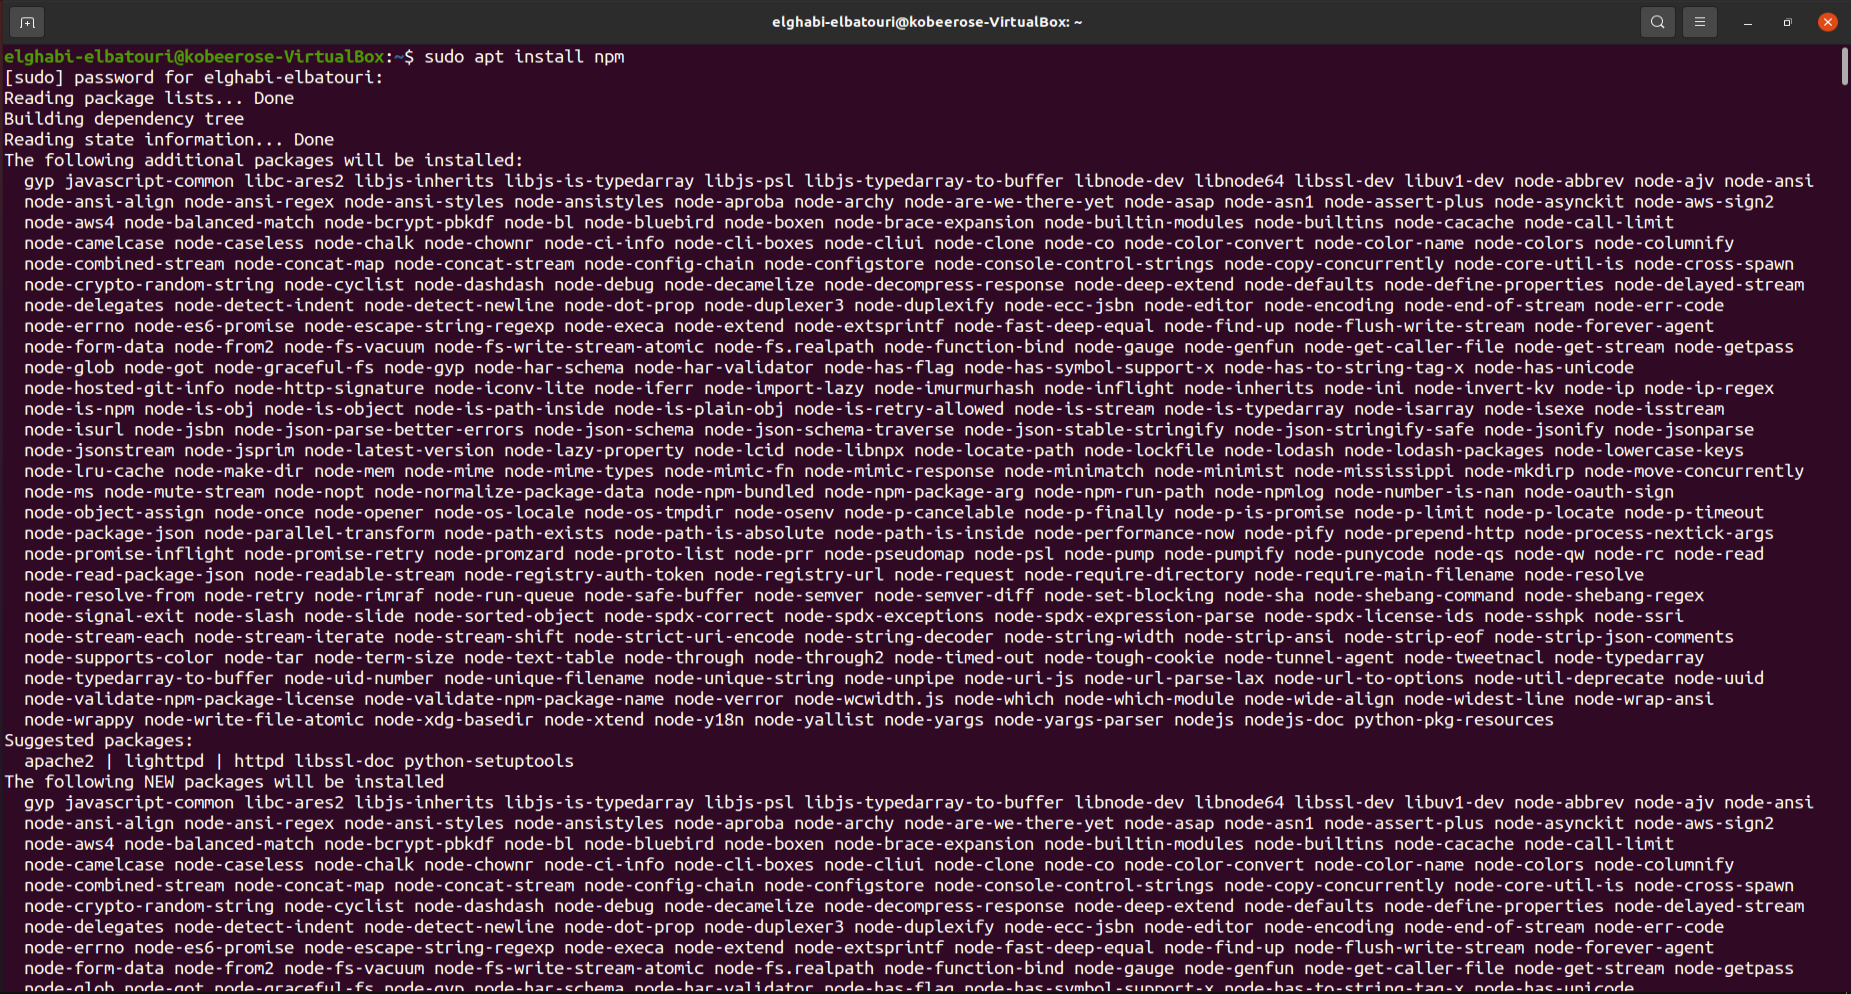
\includegraphics[width=1\linewidth]{Pictures/MongoDB/Nodejs and MongoDB CRUD application/Nodejs installation/Install npm} 
\end{center} 
\caption{Install npm} 
\end{figure}  \FloatBarrier
\\
\newpage
\par Creating a directory called “productsapp” where we will put our project. afterward we run npm init command to initialize a node project. 
\\
\begin{figure}[!htb] 
\begin{center} 
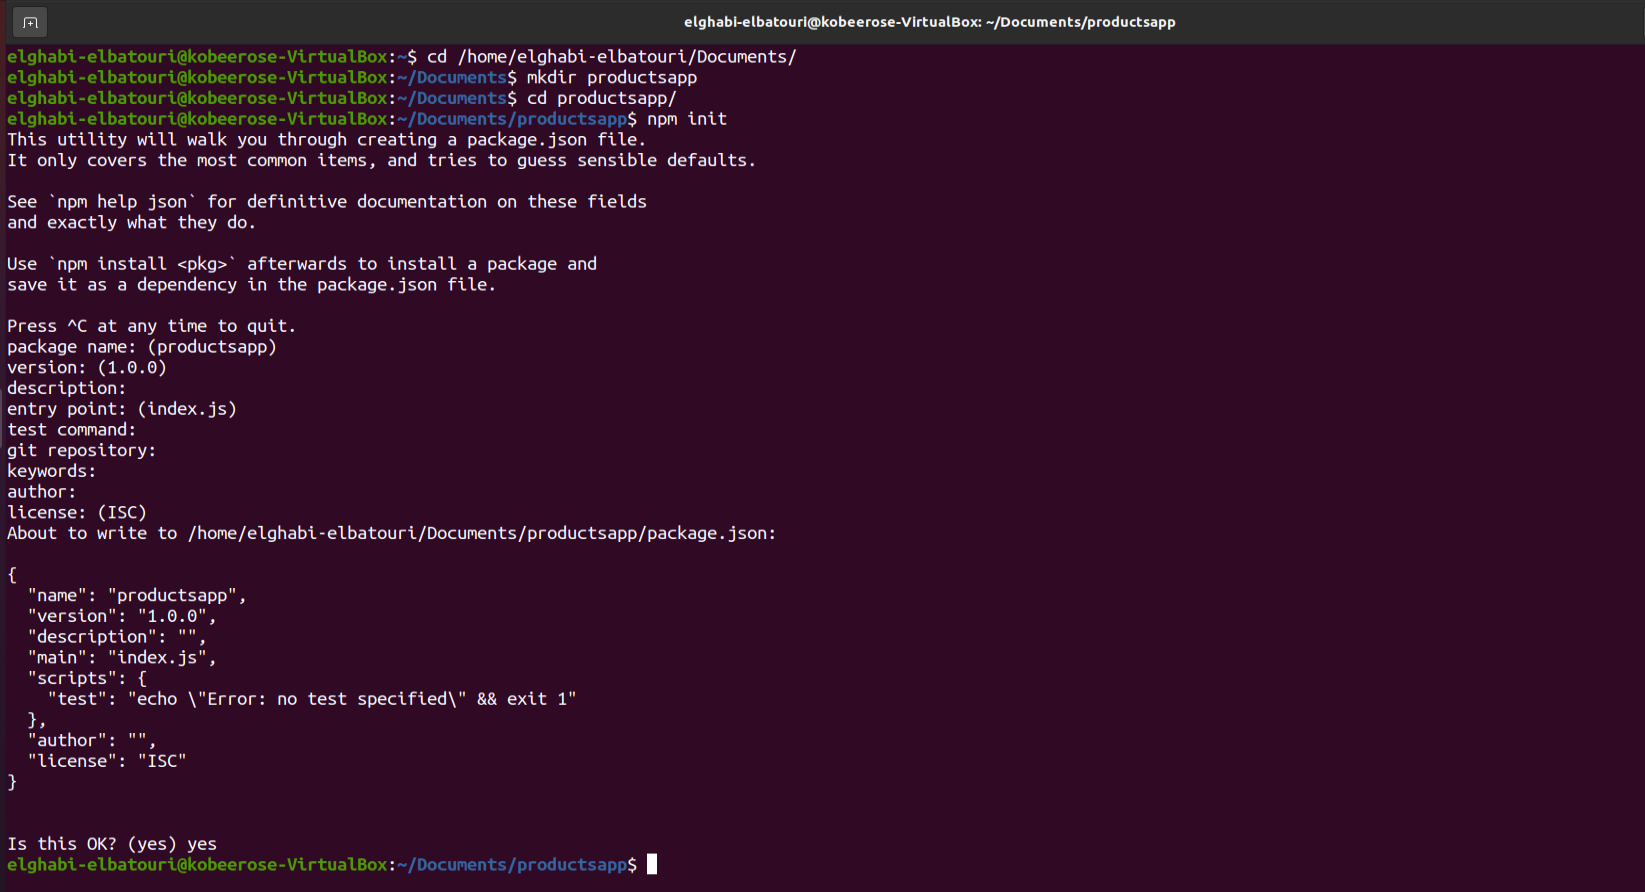
\includegraphics[width=1\linewidth]{Pictures/MongoDB/Nodejs and MongoDB CRUD  application/Nodejs installation/Creating package.json file} 
\end{center} 
\caption{Creating package.json file} 
\end{figure}  \FloatBarrier
\\

\par We will install the packages that we will use for our API which are ExpressJS, mongoose and body-parser.
\\
\begin{figure}[!htb] 
\begin{center} 
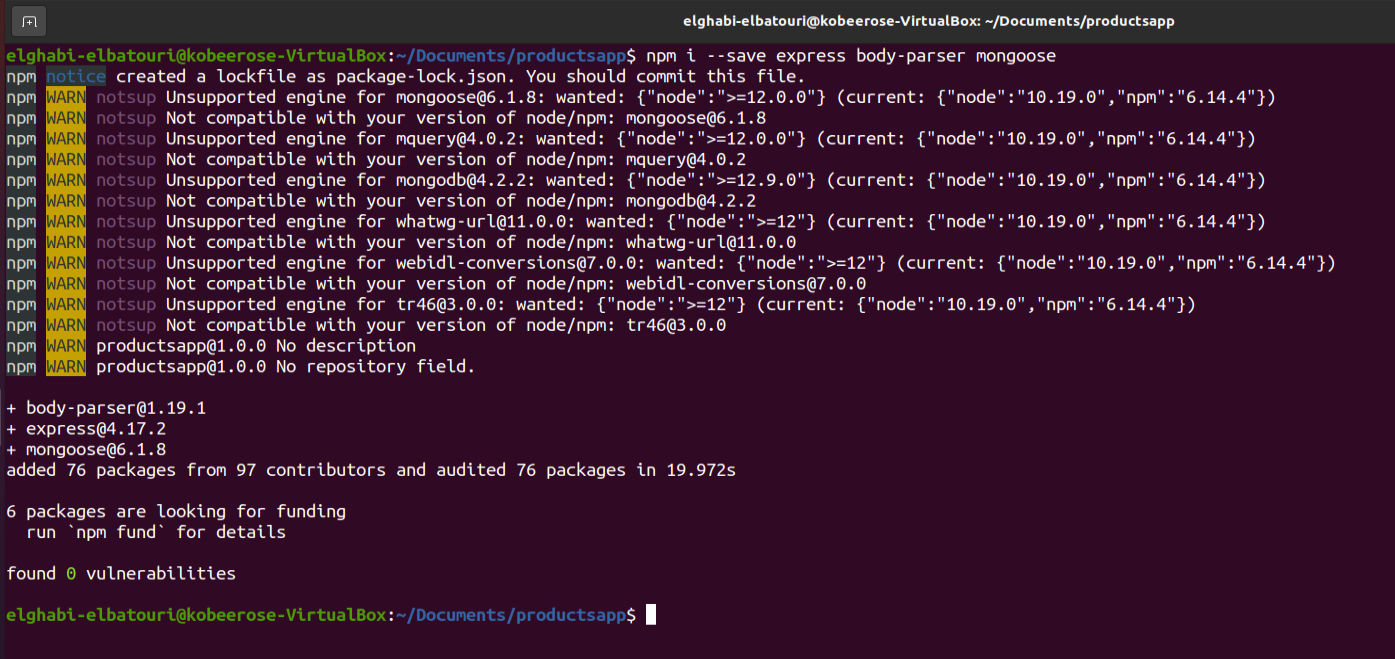
\includegraphics[width=1\linewidth]{Pictures/MongoDB/Nodejs and MongoDB CRUD  application/Nodejs installation/Installing dependencies} 
\end{center} 
\caption{Installing dependencies} 
\end{figure}  \FloatBarrier
\\
\newpage
\par We create a new file named app.js and add all previously installed dependencies.
The next step would be to dedicate a port number and tell our express app to listen
this port.
\\
\begin{figure}[!htb] 
\begin{center} 
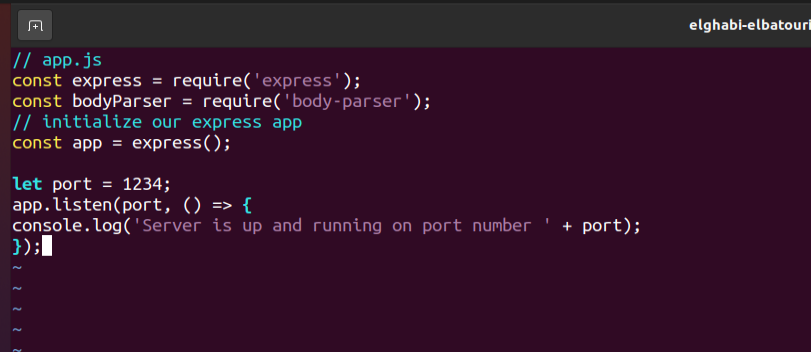
\includegraphics[width=1\linewidth]{Pictures/MongoDB/Nodejs and MongoDB CRUD  application/Nodejs installation/Creating app.js file} 
\end{center} 
\caption{Creating app.js file} 
\end{figure}  \FloatBarrier
\\

\par Now we should be able to test our server
in the terminal:
\\
\begin{figure}[!htb] 
\begin{center} 
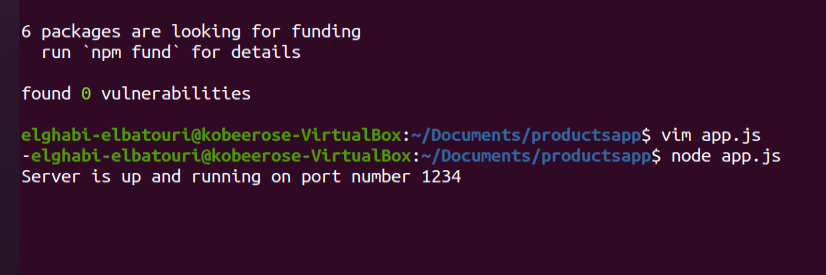
\includegraphics[width=1\linewidth]{Pictures/MongoDB/Nodejs and MongoDB CRUD  application/Nodejs installation/Running app.js} 
\end{center} 
\caption{Running app.js} 
\end{figure}  \FloatBarrier
\\

\newpage
\section{Organization of the Node Application }
\par We will be working with a design pattern called MVC. It's a good way to separate the
parts of our application and group them according to their functionality and role.\\
In the productsapp directory, we will create four subdirectories Controllers, Models, Routes, Viewss
\\
\begin{figure}[!htb] 
\begin{center} 
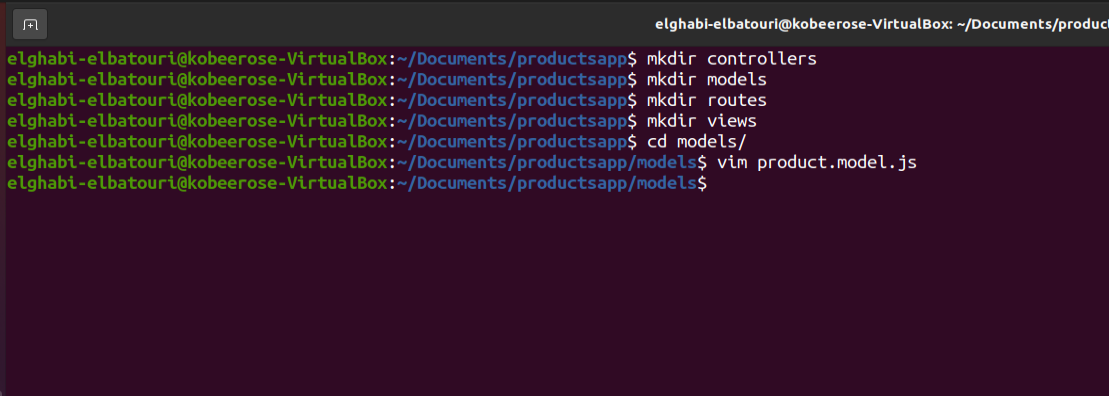
\includegraphics[width=1\linewidth]{Pictures/MongoDB/Nodejs and MongoDB CRUD  application/Organization of the Node Application/Repositories for the app} 
\end{center} 
\caption{Repositories for the app} 
\end{figure}  \FloatBarrier
\\

\par In MVC M stands for Models, which will include all code for our database models (
in this case will be products).\\ We will start by defining our model and creating a new file in the directory
“models” and call it “product.model.js”.
\\
\begin{figure}[!htb] 
\begin{center} 
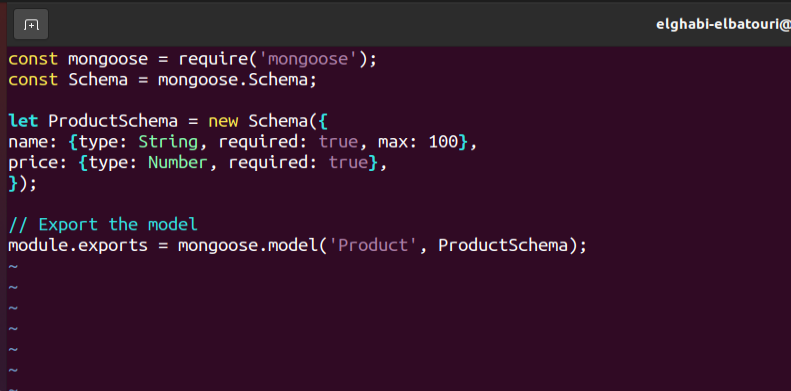
\includegraphics[width=1\linewidth]{Pictures/MongoDB/Nodejs and MongoDB CRUD  application/Organization of the Node Application/Creating product.model.js file} 
\end{center} 
\caption{Creating product.model.js file} 
\end{figure}  \FloatBarrier
\\
\newpage
\par Routes, they tell the client (browser / mobile app)
to go to which controller once a specific URL/path is requested. In the routes directory, we create a “product.route.js” file that will contain the product routes.
\\
\begin{figure}[!htb] 
\begin{center} 
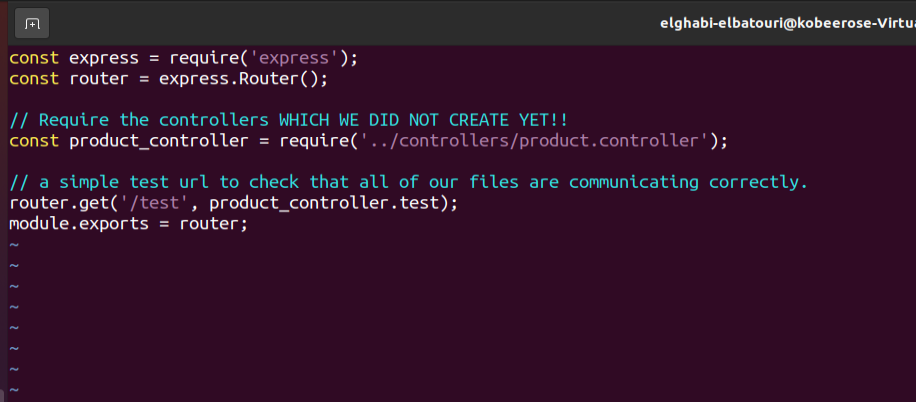
\includegraphics[width=1\linewidth]{Pictures/MongoDB/Nodejs and MongoDB CRUD  application/Organization of the Node Application/Creating product.route.js file} 
\end{center} 
\caption{Creating product.route.js file} 
\end{figure}  \FloatBarrier
\\

\par In MVC, the letter C stands for controllers, which is the logic of how the application handles requests incoming and outgoing responses.The next step is to implement the controllers we referenced in roads. therefore create a new file named product.controller.js which will be the placeholder for our controllers.
\\
\begin{figure}[!htb] 
\begin{center} 
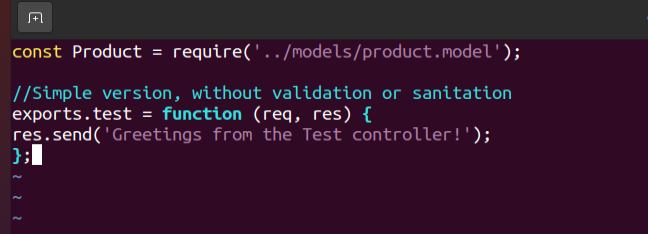
\includegraphics[width=1\linewidth]{Pictures/MongoDB/Nodejs and MongoDB CRUD  application/Organization of the Node Application/Creating product.controller.js file} 
\end{center} 
\caption{Creating product.controller.js file} 
\end{figure}  \FloatBarrier
\\
\newpage
\par The last step before trying our first route is to add the route class to app.js file.
\\
\begin{figure}[!htb] 
\begin{center} 
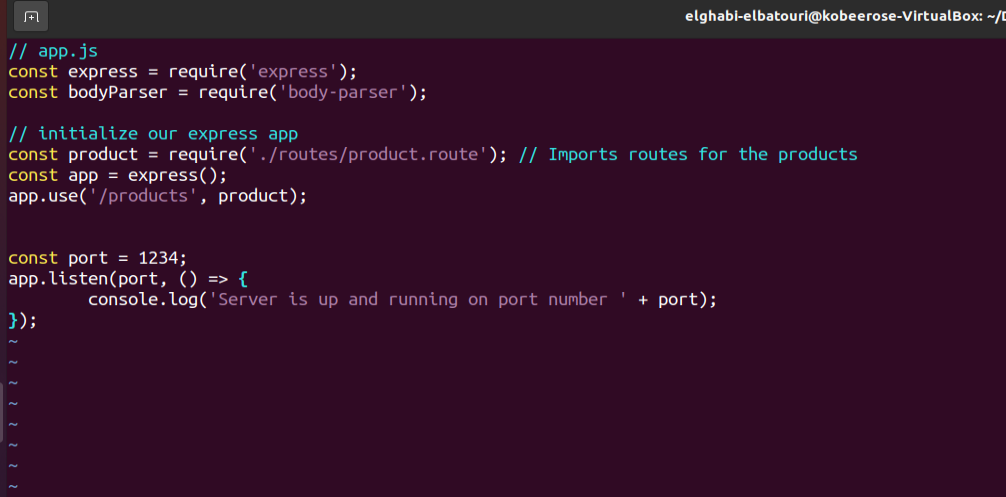
\includegraphics[width=1\linewidth]{Pictures/MongoDB/Nodejs and MongoDB CRUD  application/Organization of the Node Application/Adding route to the app} 
\end{center} 
\caption{Adding route to the app} 
\end{figure}  \FloatBarrier
\\

\par We try to run the application but, there is an error that appears.
\\
\begin{figure}[!htb] 
\begin{center} 
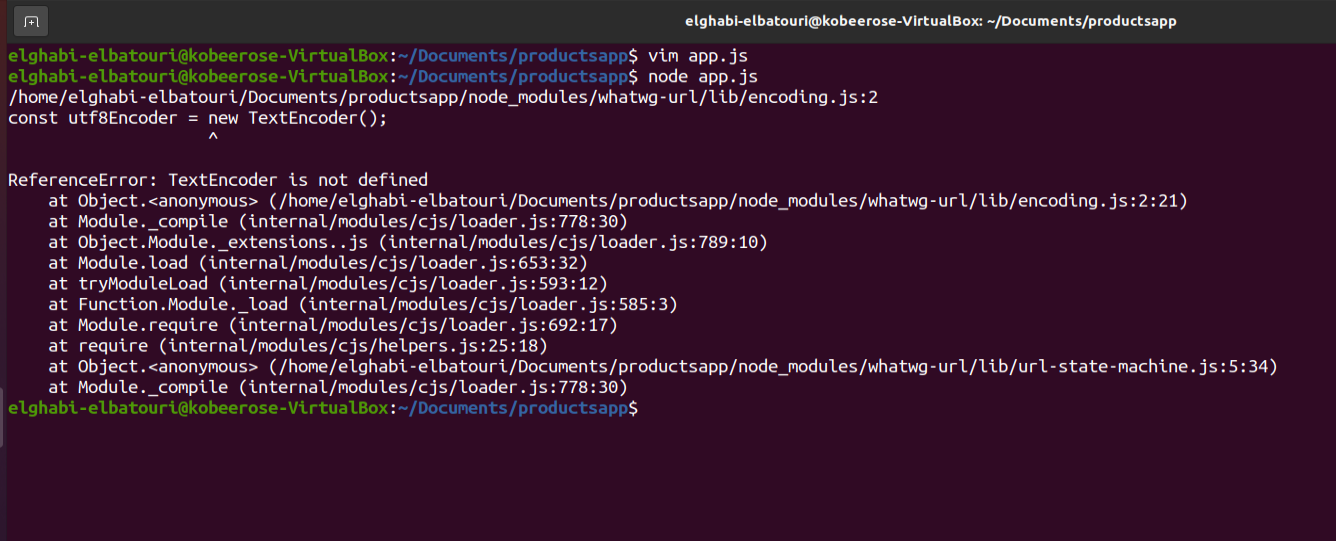
\includegraphics[width=1\linewidth]{Pictures/MongoDB/Nodejs and MongoDB CRUD  application/Organization of the Node Application/Error when running the app} 
\end{center} 
\caption{Error when running the app} 
\end{figure}  \FloatBarrier
\\
\newpage
\par In order to fix it, We need to make some changes to the encoding.js file.
\\
\begin{figure}[!htb] 
\begin{center} 
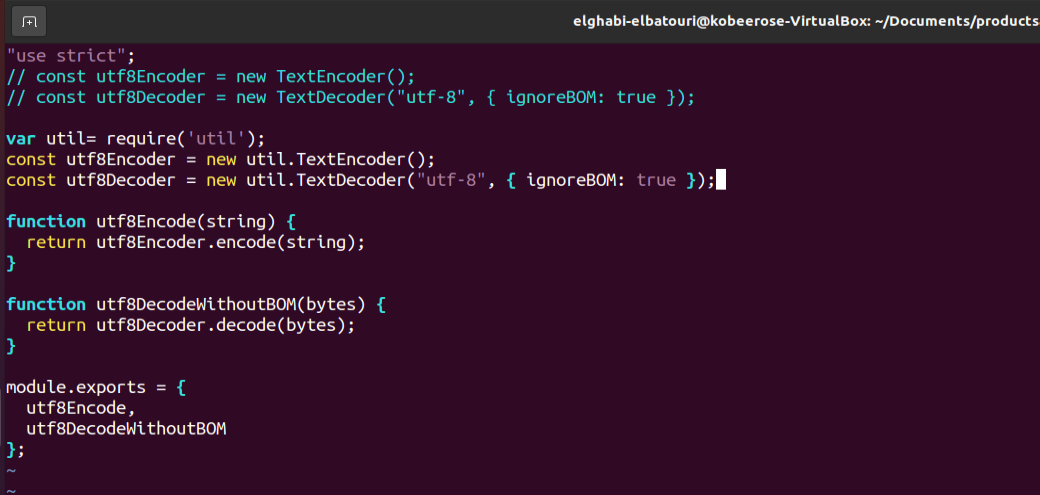
\includegraphics[width=1\linewidth]{Pictures/MongoDB/Nodejs and MongoDB CRUD  application/Organization of the Node Application/Modifying encoding.js file} 
\end{center} 
\caption{Modifying encoding.js file} 
\end{figure}  \FloatBarrier
\\
\par Finally we run the application and head to our browser and try it out.
\\
\begin{figure}[!htb] 
\begin{center} 
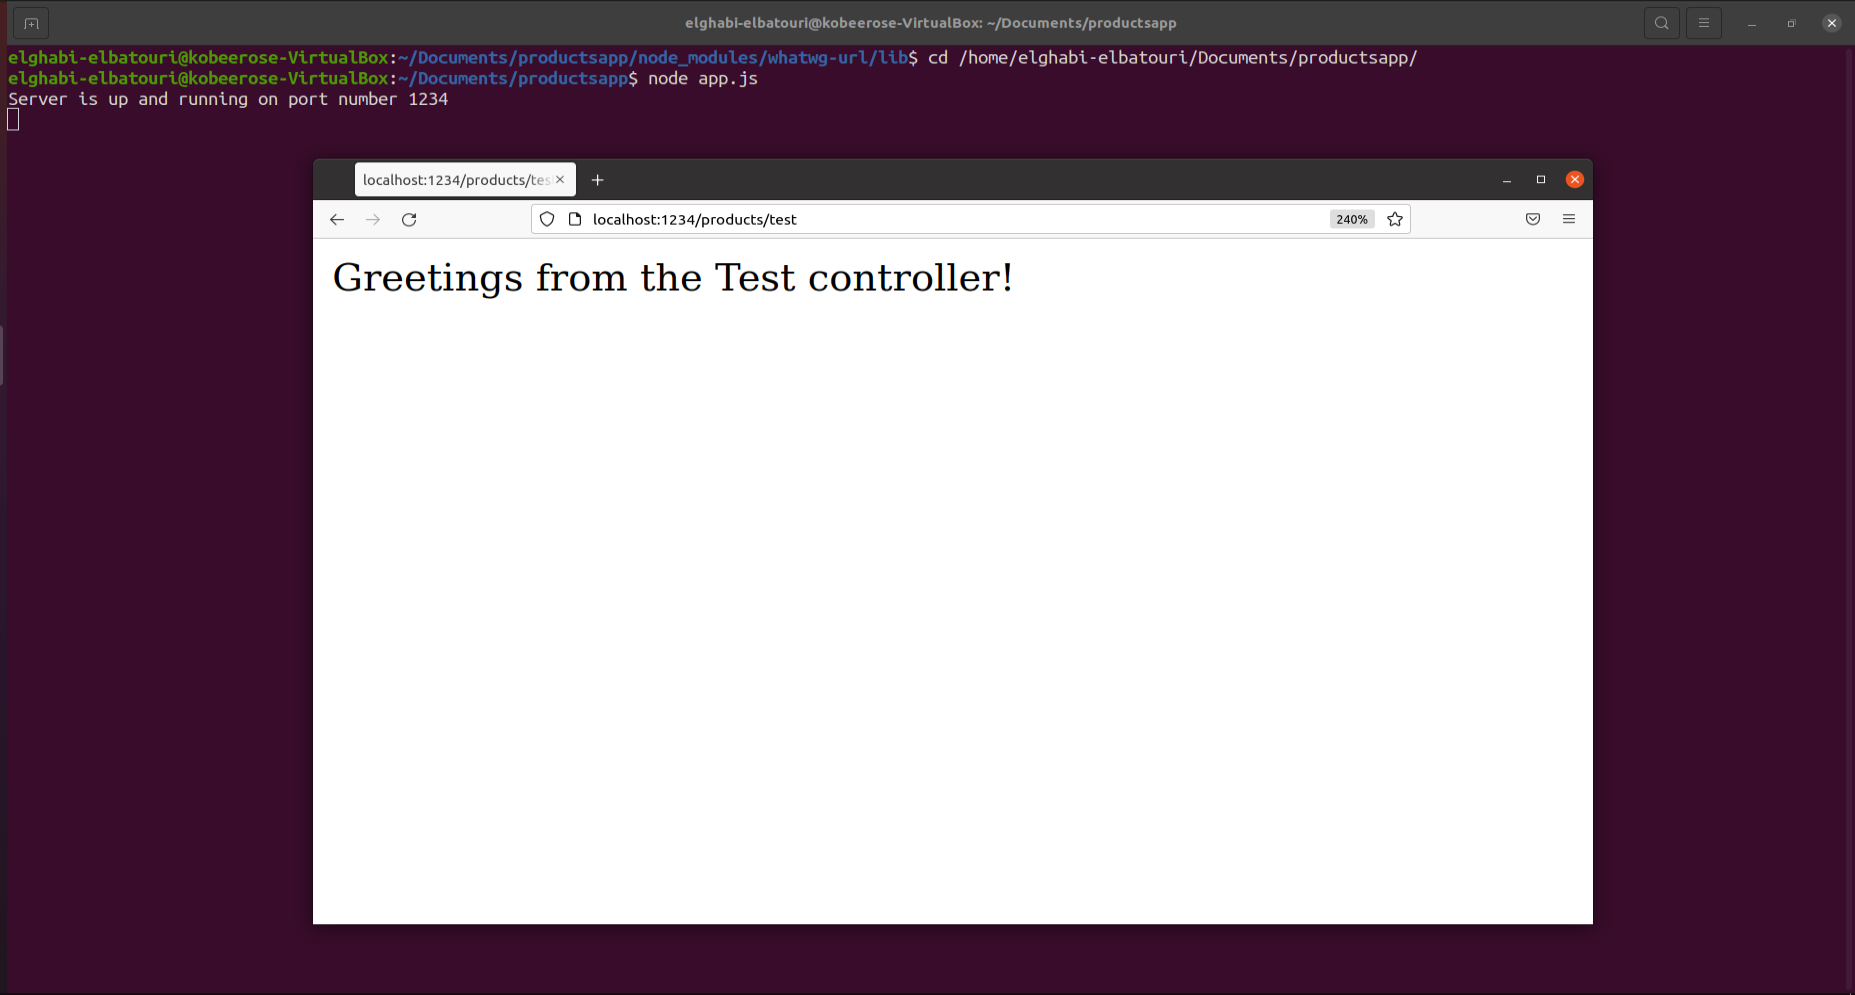
\includegraphics[width=1\linewidth]{Pictures/MongoDB/Nodejs and MongoDB CRUD  application/Organization of the Node Application/Testing the app in browser} 
\end{center} 
\caption{Testing the app in browser} 
\end{figure}  \FloatBarrier
\\

\newpage
\section{Postman }
\par Postman is a very powerful HTTP client used for testing, documentation and development
of APIs. We will use Postman here to test our endpoints which we will implement in this
PT. But first, we will install and test Postman.

\begin{figure}[!htb] 
\begin{center} 
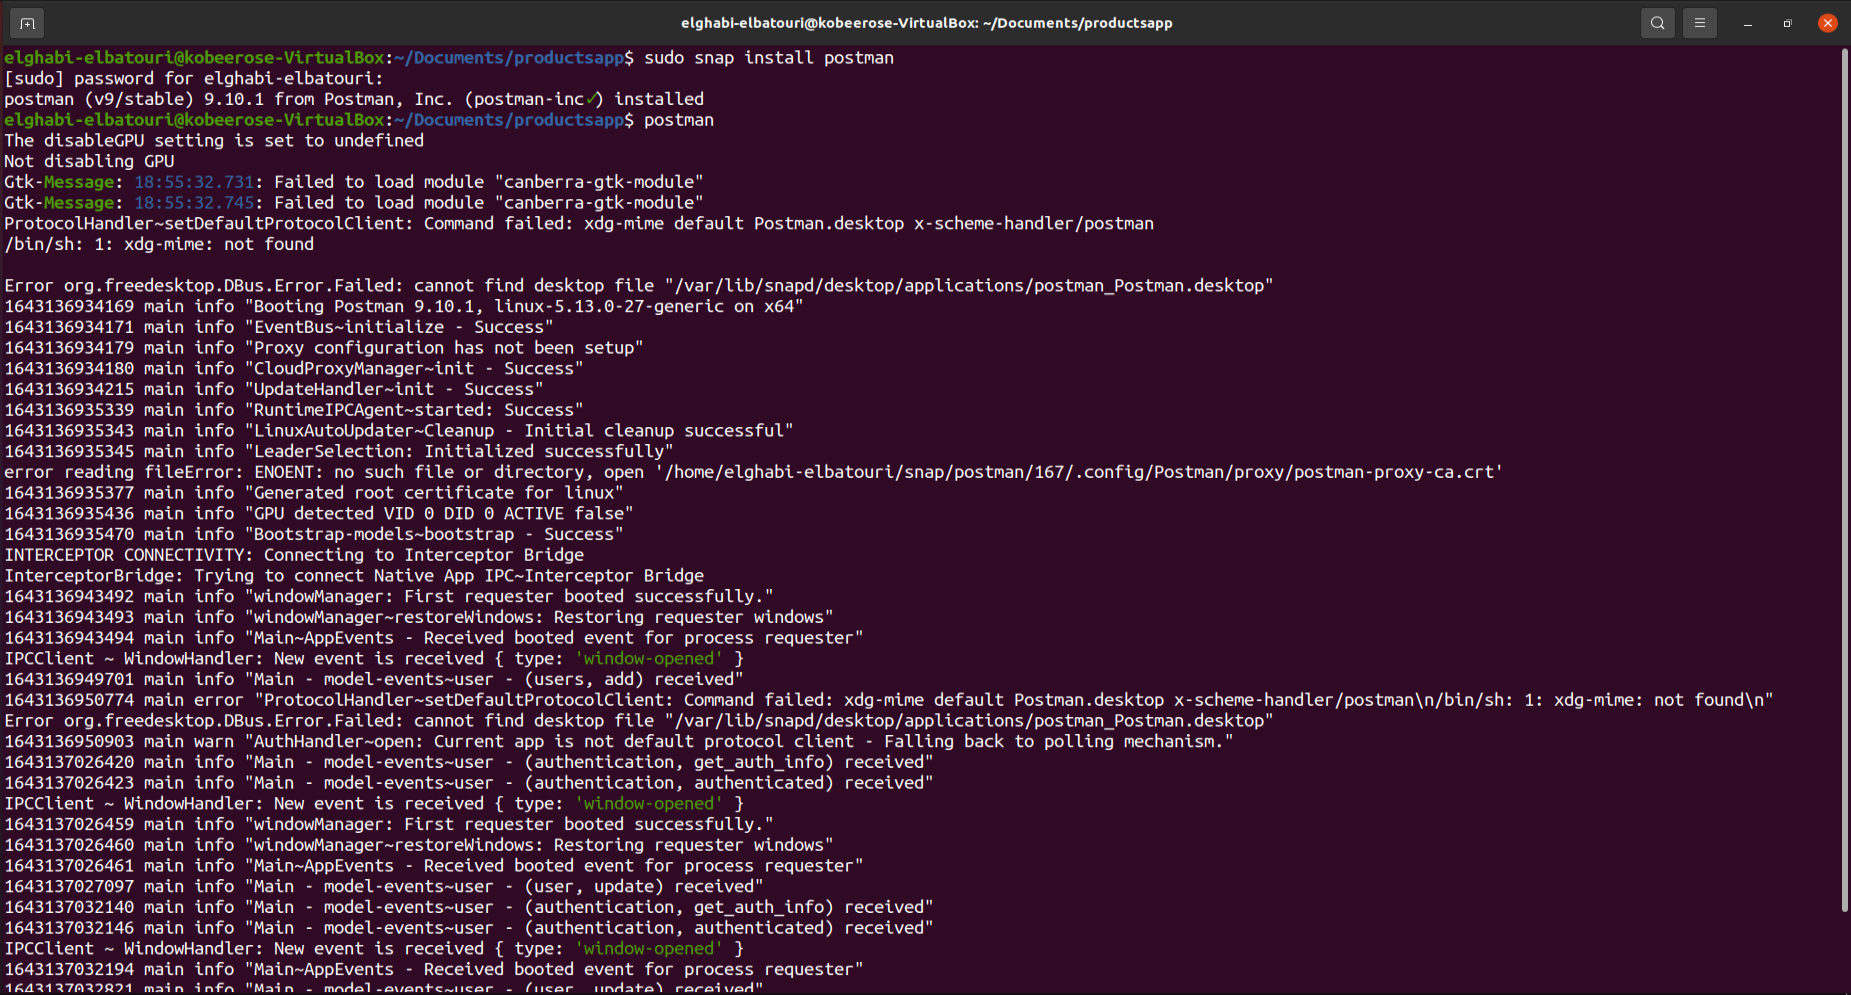
\includegraphics[width=.95\linewidth]{Pictures/MongoDB/Nodejs and MongoDB CRUD  application/Postman/Installing and running Postman} 
\end{center} 
\caption{Installing and running Postman} 
\end{figure}  \FloatBarrier
\\

\par Let's create a “GET request to the following url: “localhost:1234/products/test and check the results in postman.
\begin{figure}[!htb] 
\begin{center} 
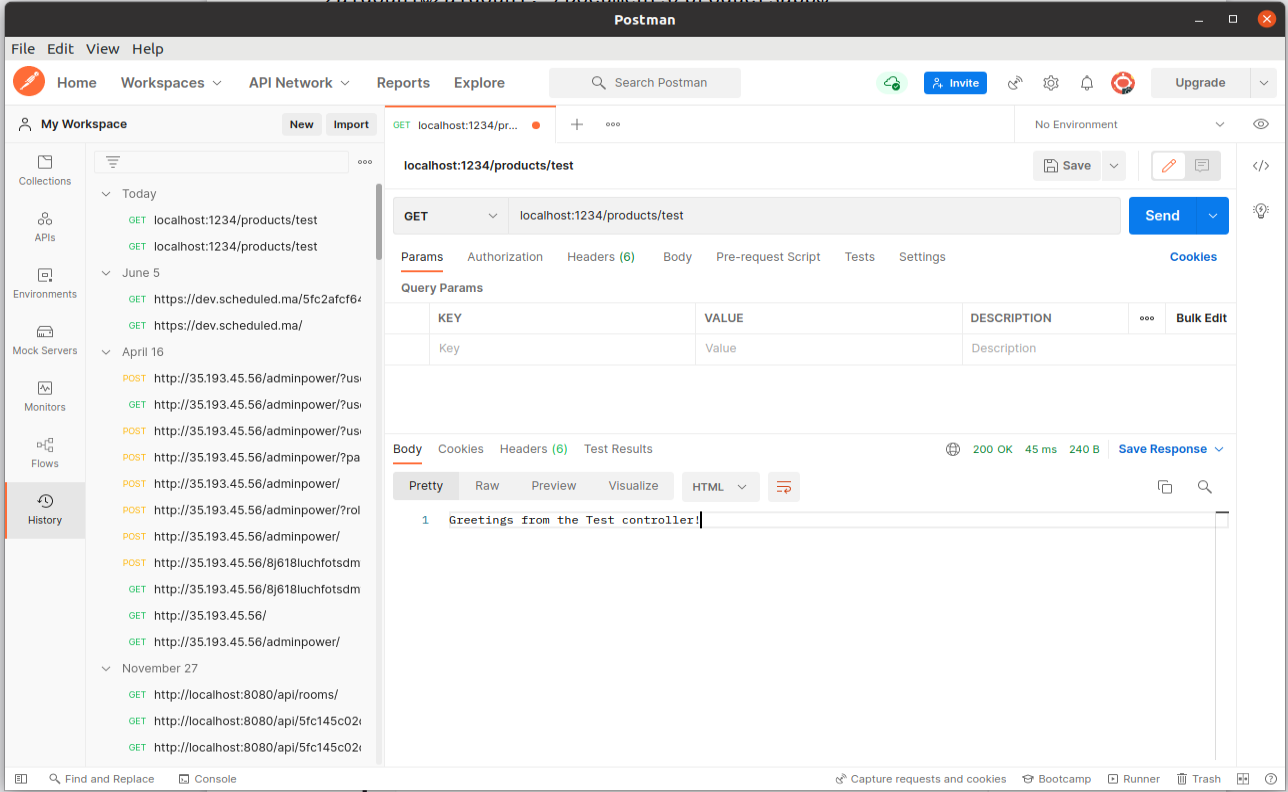
\includegraphics[width=.95\linewidth]{Pictures/MongoDB/Nodejs and MongoDB CRUD  application/Postman/Testing GET request with Postman} 
\end{center} 
\caption{Testing GET request with Postman} 
\end{figure}  \FloatBarrier
\\

\par We need to inform our application that it needs to communicate with the database. So we will use the package already installed "mongoose".
\\
\begin{figure}[!htb] 
\begin{center} 
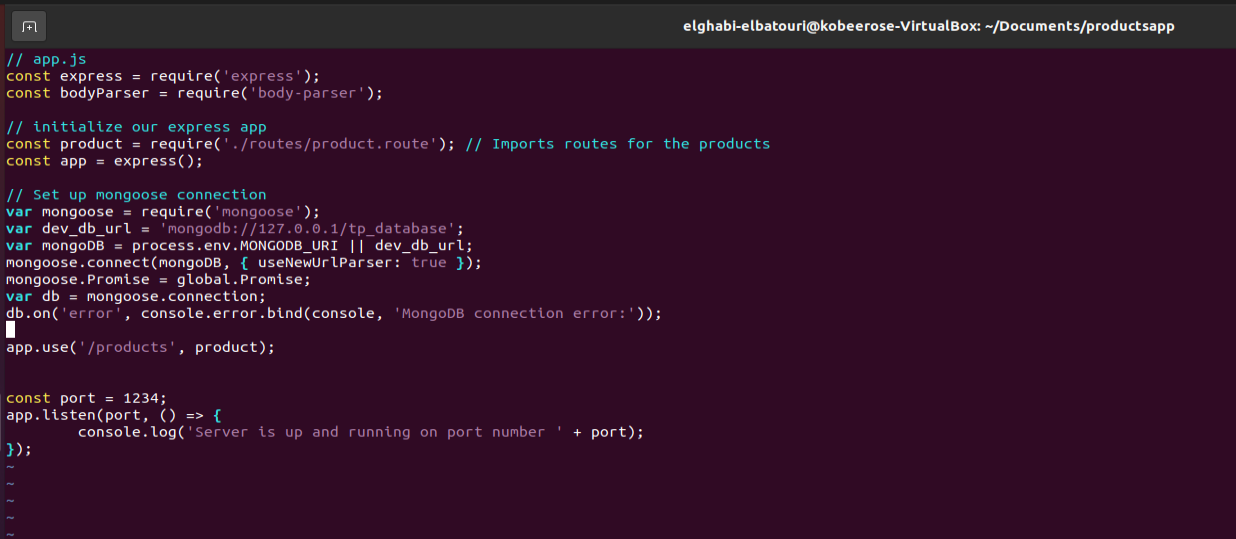
\includegraphics[width=1\linewidth]{Pictures/MongoDB/Nodejs and MongoDB CRUD  application/Postman/Connection to mongoose} 
\end{center} 
\caption{Connection to mongoose} 
\end{figure}  \FloatBarrier
\\

\par The last thing we need for our setup is to use the “bodyParser”.
Body Parser is an npm package used to parse request bodies in middleware.
\\
\begin{figure}[!htb] 
\begin{center} 
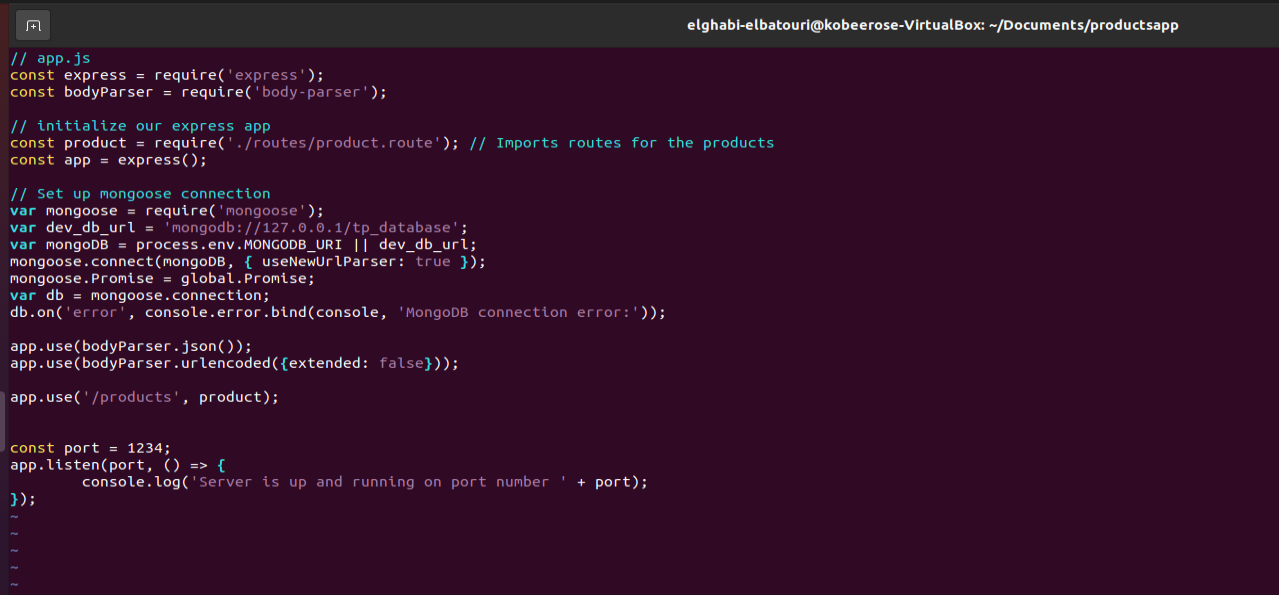
\includegraphics[width=1\linewidth]{Pictures/MongoDB/Nodejs and MongoDB CRUD  application/Postman/Body Parser package} 
\end{center} 
\caption{Body Parser package} 
\end{figure}  \FloatBarrier
\\

\newpage
\section{Implementing Endpoints }
\par The first task of our CRUD operations is to create a new product. Let's start with
define our route then we create the product\_create controller.
\begin{figure}[!htb] 
\begin{center} 
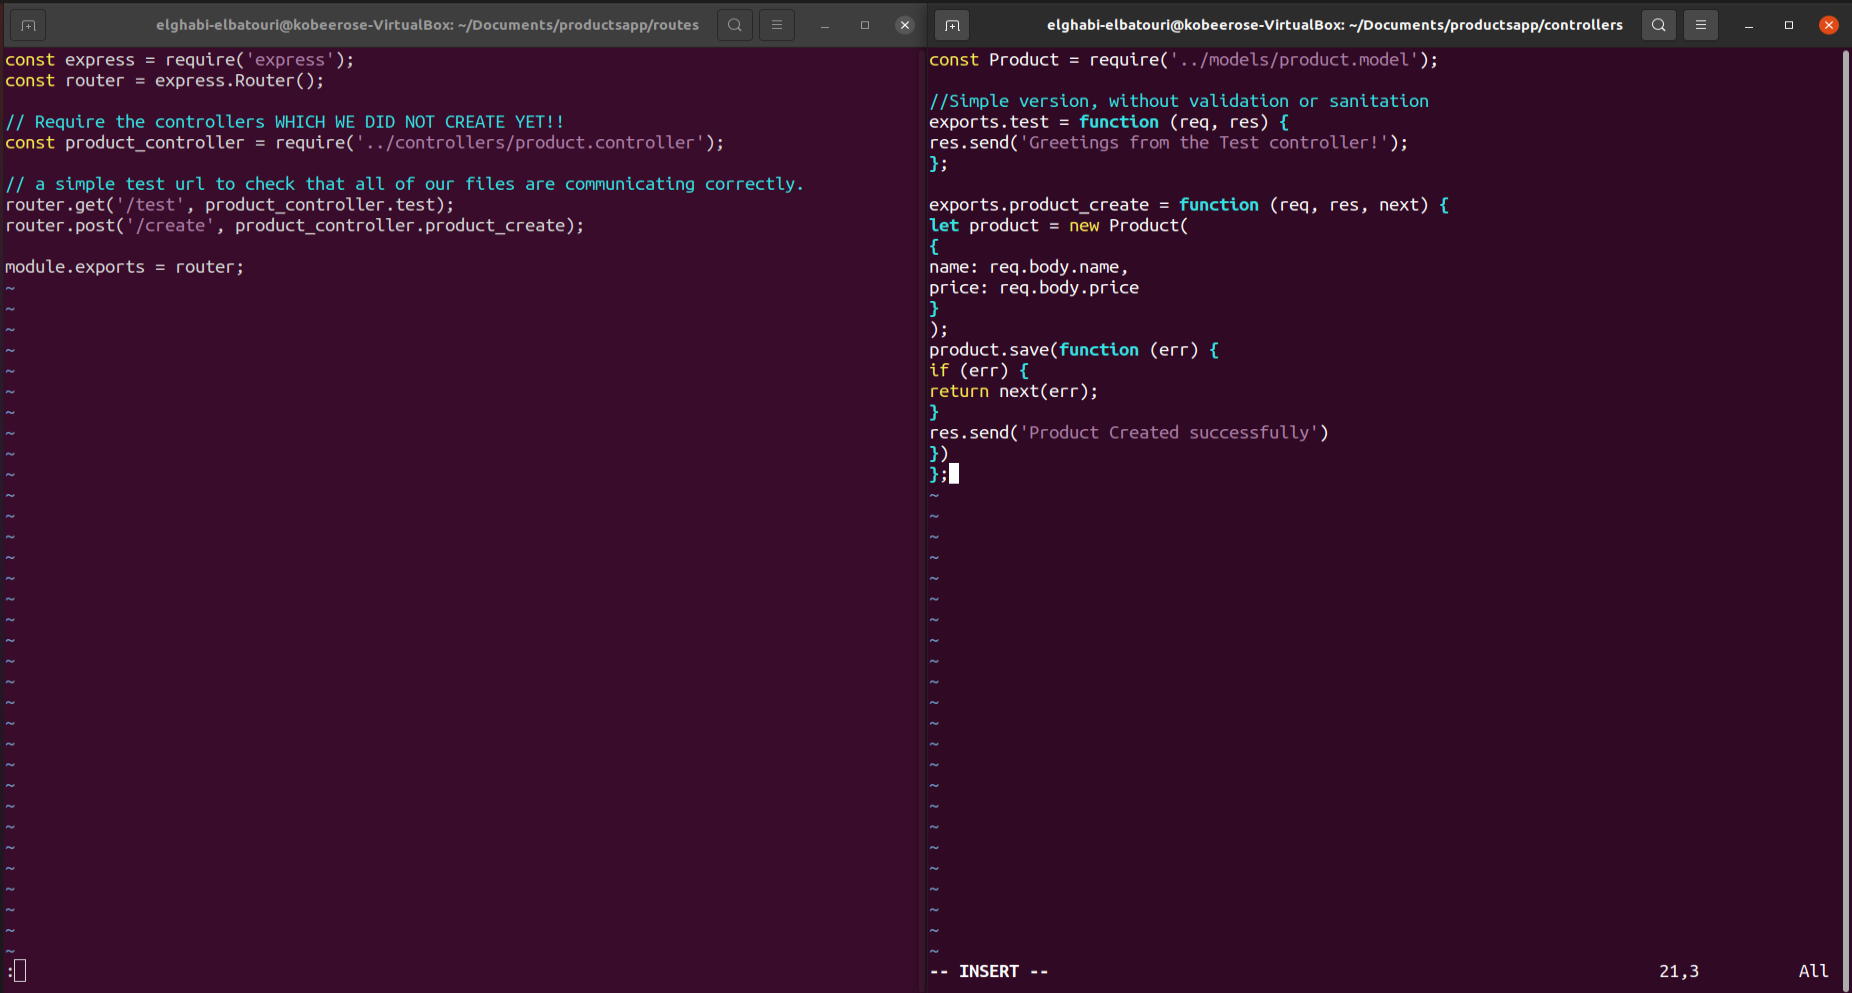
\includegraphics[width=.97\linewidth]{Pictures/MongoDB/Nodejs and MongoDB CRUD  application/Implementing Endpoints/Router and Controller for CREATE} 
\end{center} 
\caption{Router and Controller for CREATE} 
\end{figure}  \FloatBarrier
\\
\par We test our endpoint by sending a POST request to the following URL: "localhost:1234/products/create" and
specifying the POST data. like ( name: apple, price: 15 )...
\begin{figure}[!htb] 
\begin{center} 
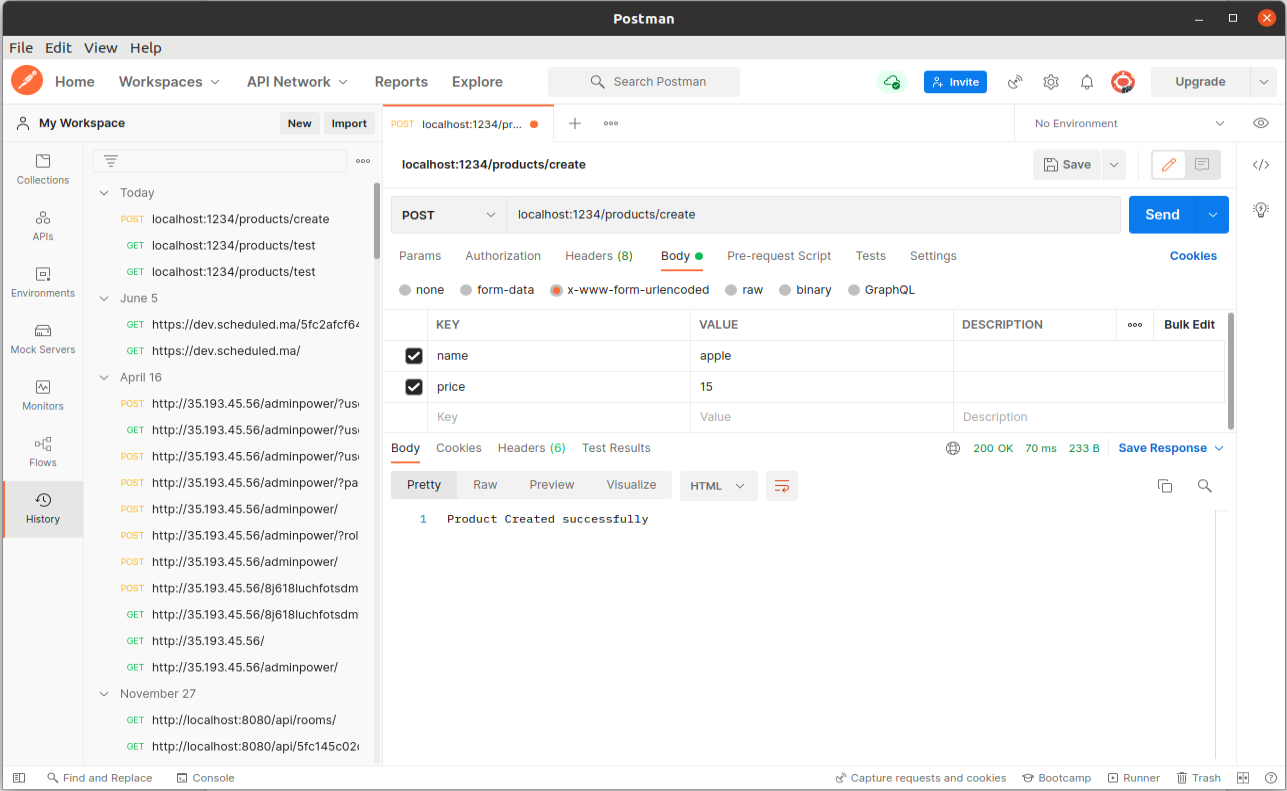
\includegraphics[width=.97\linewidth]{Pictures/MongoDB/Nodejs and MongoDB CRUD  application/Implementing Endpoints/Testing CREATE endpoint} 
\end{center} 
\caption{Testing CREATE endpoint} 
\end{figure}  \FloatBarrier
\\

\par To verify again that an "apple" product was created,
Let's check the database. we first connect to the Mongo terminal and check that a
table named: "tp\_database" and a collection "products" are well created.
\\
\begin{figure}[!htb] 
\begin{center} 
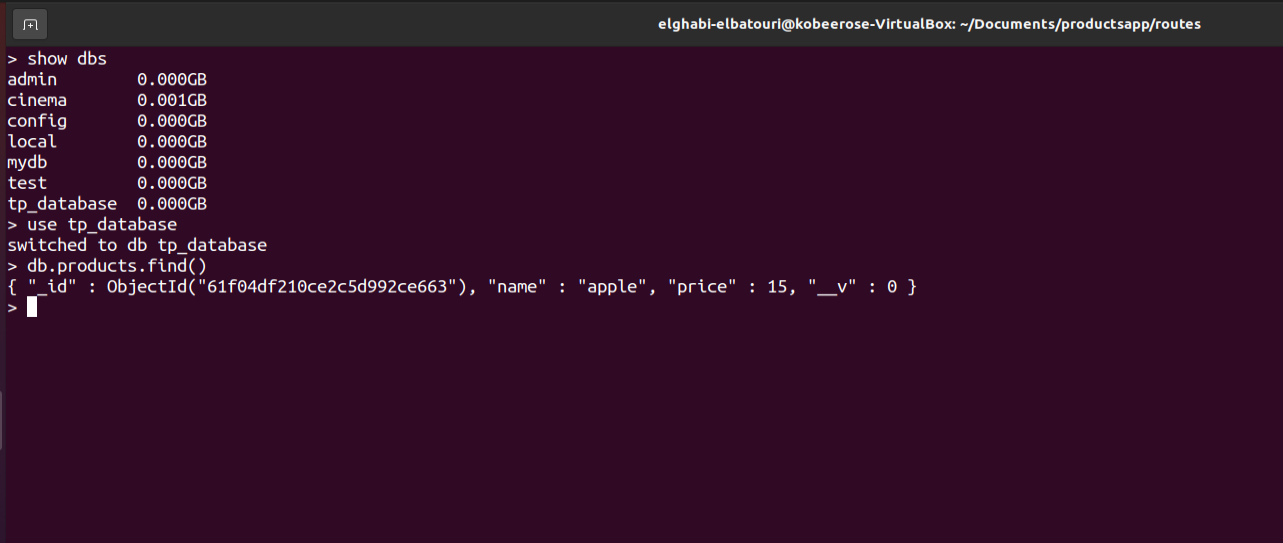
\includegraphics[width=1\linewidth]{Pictures/MongoDB/Nodejs and MongoDB CRUD  application/Implementing Endpoints/Finding new object in MongoDB} 
\end{center} 
\caption{Finding the new object in MongoDB} 
\end{figure}  \FloatBarrier
\\

\par The second task of our CRUD app is to read an existing product.
To configure the route then we create the product\_details controller.
\\
\begin{figure}[!htb] 
\begin{center} 
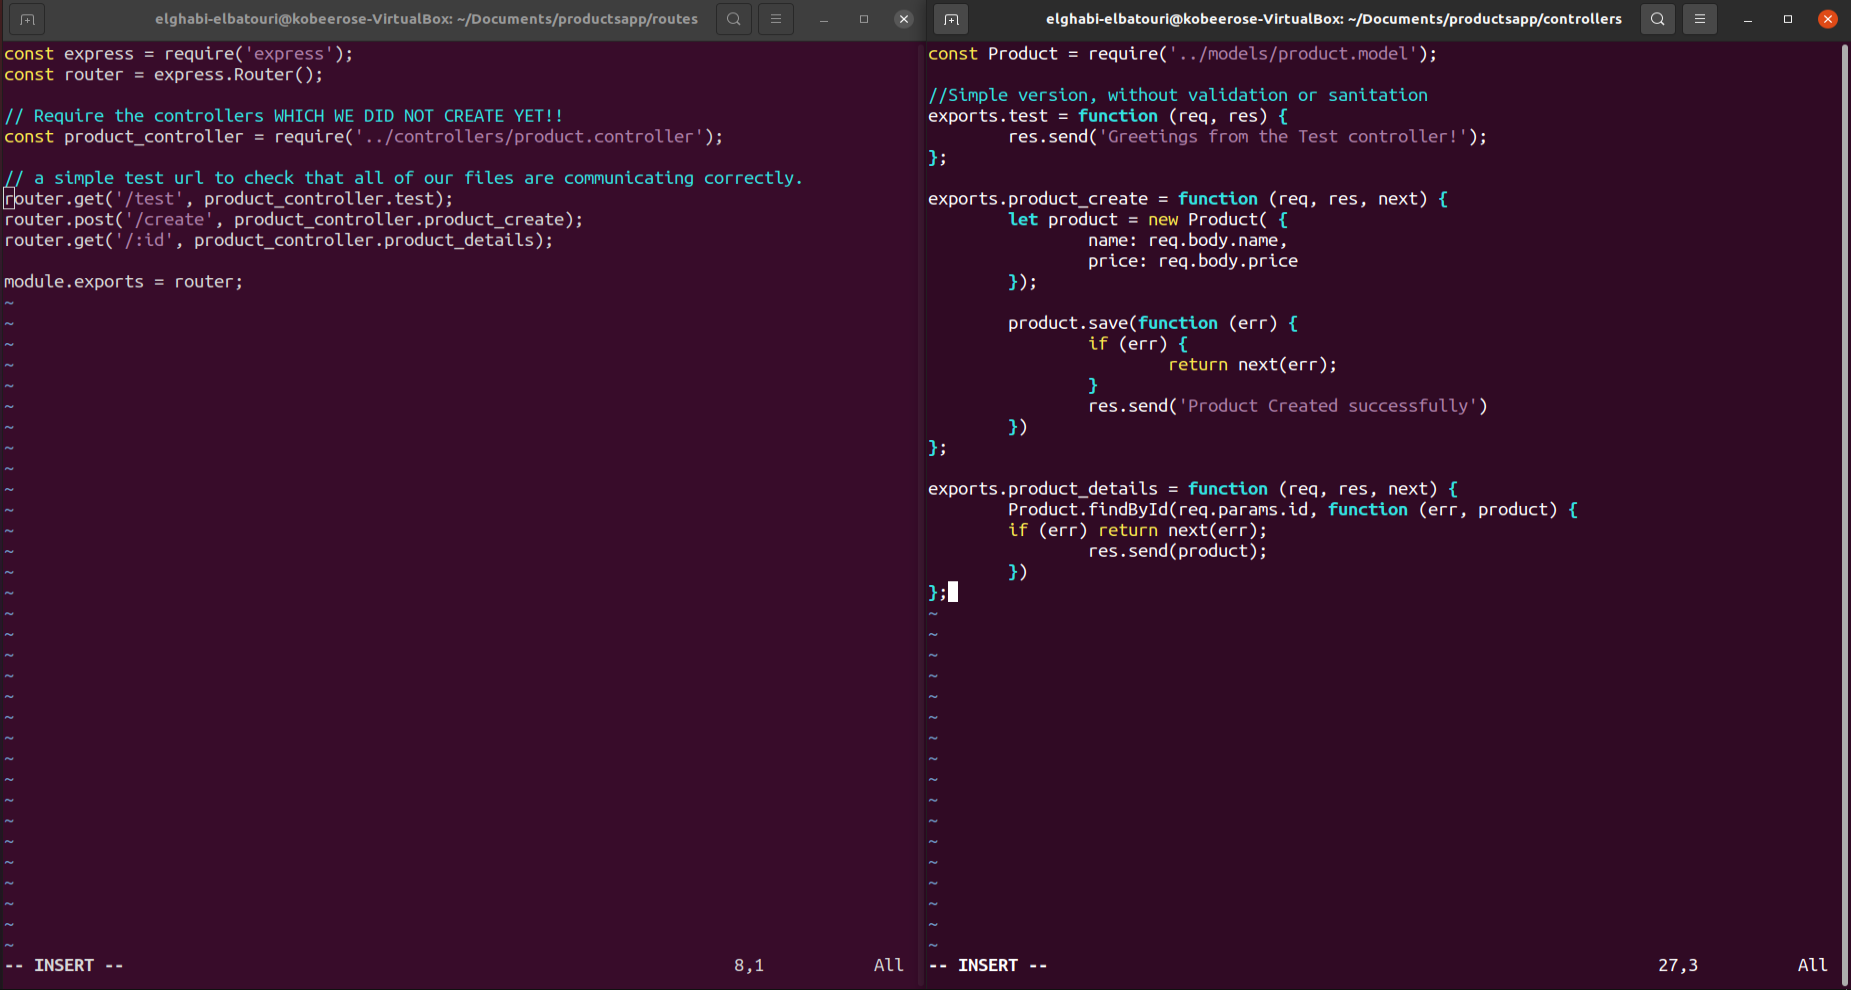
\includegraphics[width=1\linewidth]{Pictures/MongoDB/Nodejs and MongoDB CRUD  application/Implementing Endpoints/Router and Controller for READ} 
\end{center} 
\caption{Router and Controller for READ} 
\end{figure}  \FloatBarrier
\\\newpage
\par We try our new Endpoint. Choose “GET” and call the following URL:
“localhost:1234/products/PRODUCT\_ID”.
PRODUC\_ID is the ID of the object we created in the previous Endpoint.

\begin{figure}[!htb] 
\begin{center} 
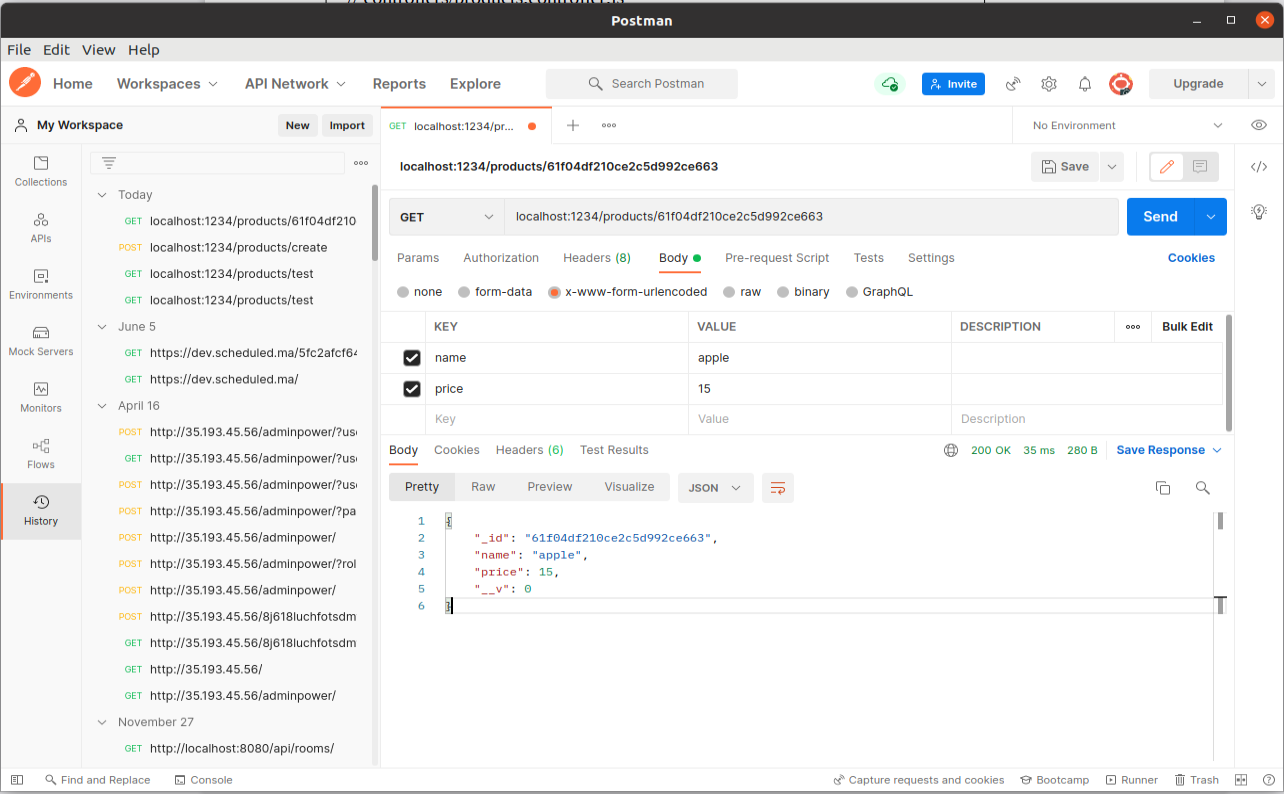
\includegraphics[width=1\linewidth]{Pictures/MongoDB/Nodejs and MongoDB CRUD  application/Implementing Endpoints/Testing READ endpoint} 
\end{center} 
\caption{Testing READ endpoint} 
\end{figure}  \FloatBarrier
\\

\par The third task of our CRUD app is to read an existing product.
To configure the route then we create the product\_update controller.
\begin{figure}[!htb] 
\begin{center} 
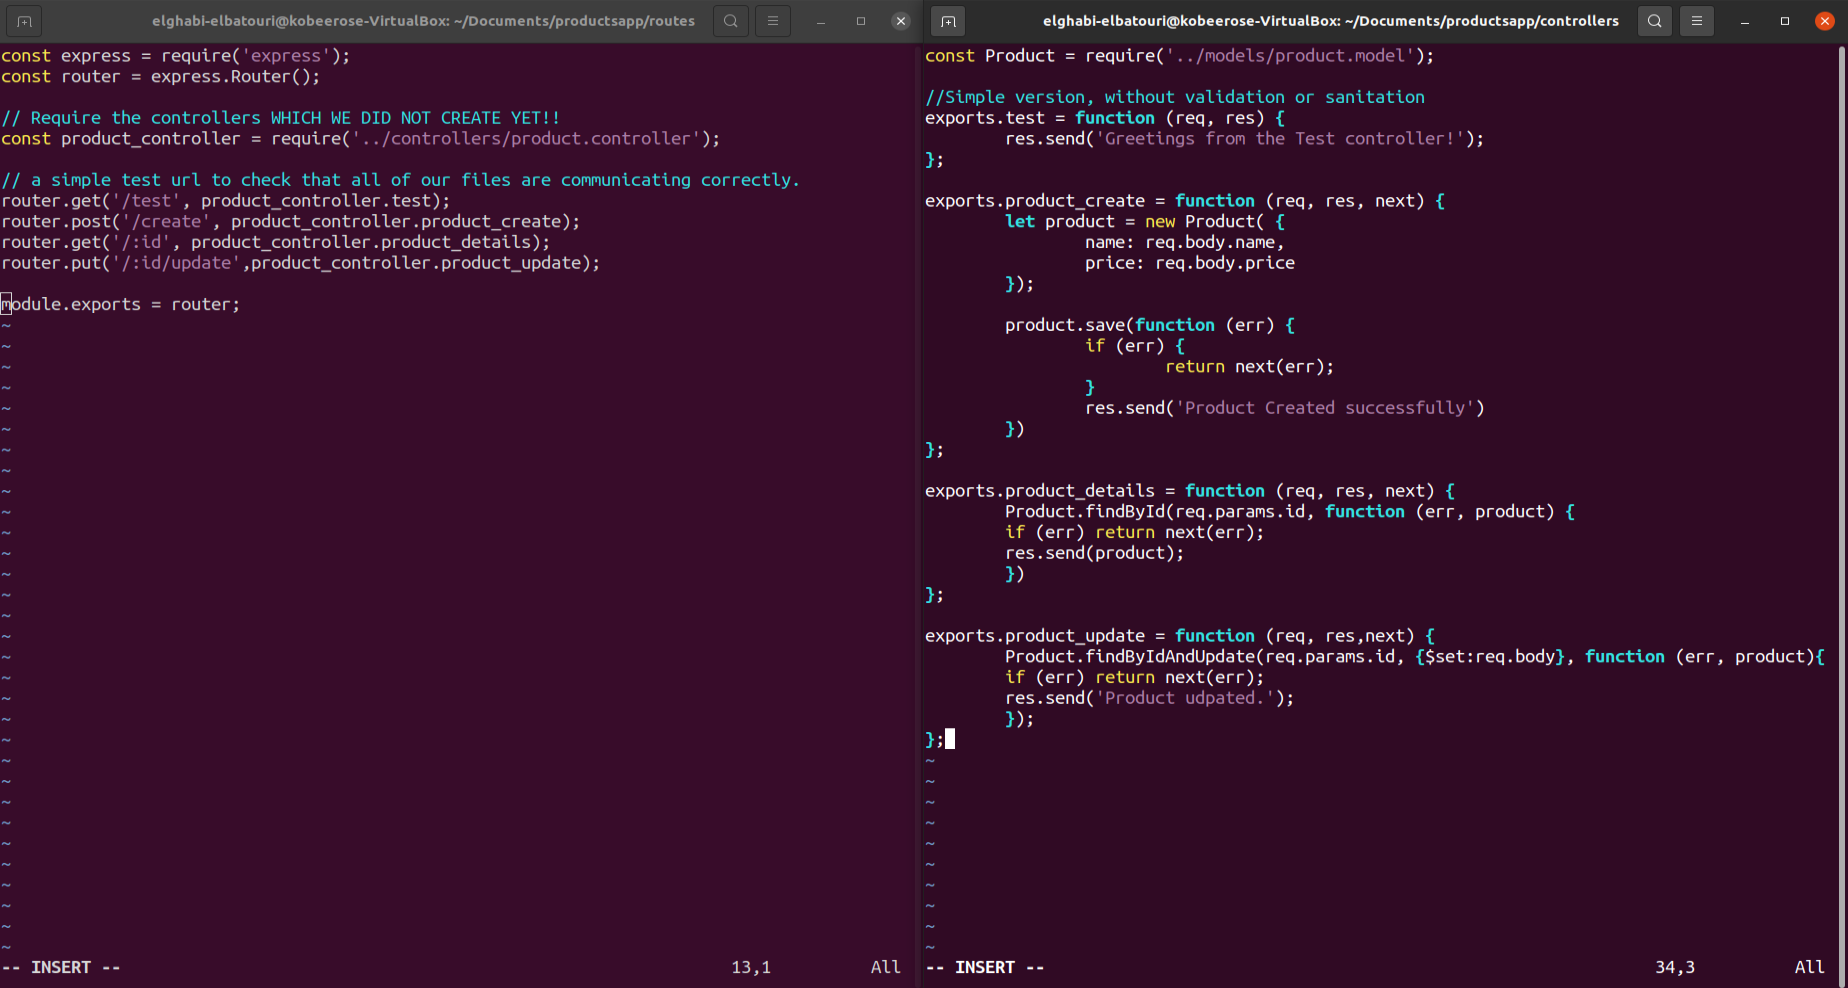
\includegraphics[width=1\linewidth]{Pictures/MongoDB/Nodejs and MongoDB CRUD  application/Implementing Endpoints/Router and Controller for UPDATE} 
\end{center} 
\caption{Router and Controller for UPDATE} 
\end{figure}  \FloatBarrier
\\
\newpage
\par Again we try our new Endpoint. Choose "PUT" and call the URL
“localhost:1234/products/PRODUCT\_ID/update”
PRODUCT\_ID is the ID of the object we created in the previous endpoint.
\\
\begin{figure}[!htb] 
\begin{center} 
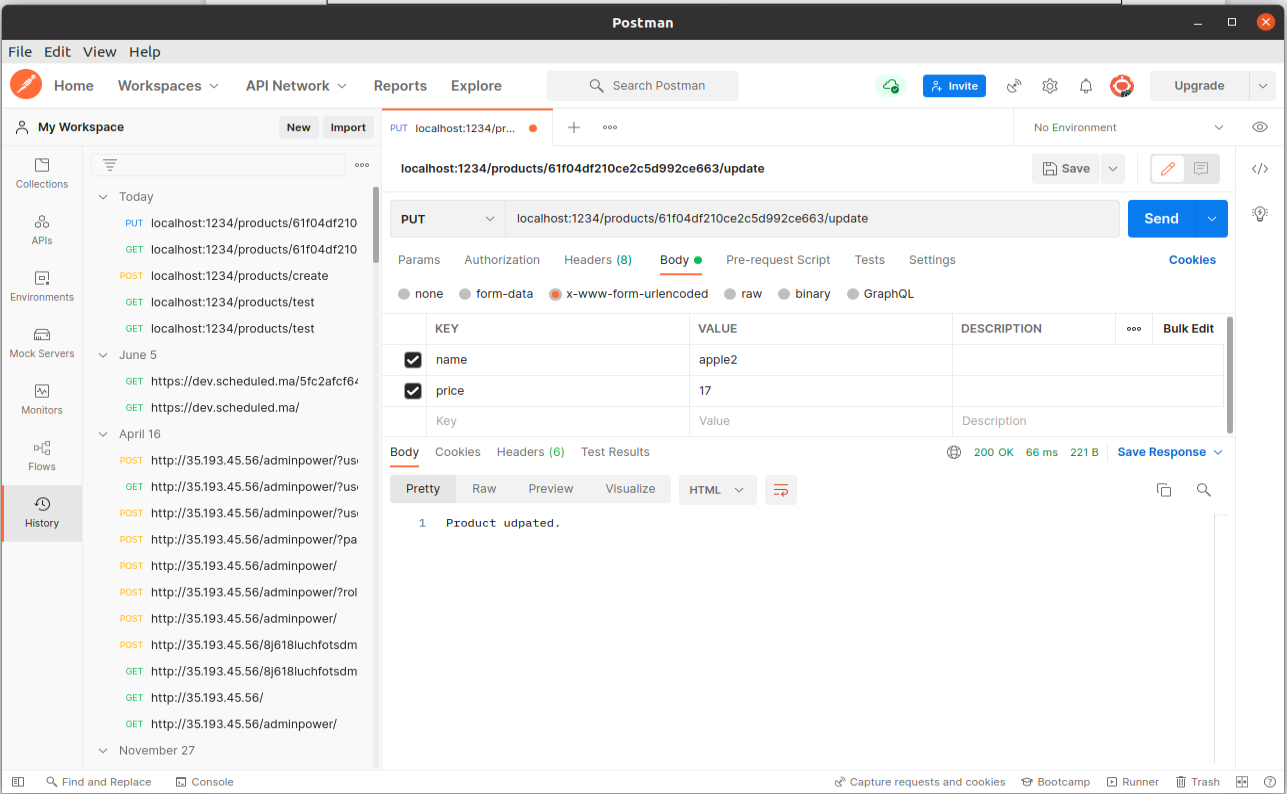
\includegraphics[width=1\linewidth]{Pictures/MongoDB/Nodejs and MongoDB CRUD  application/Implementing Endpoints/Testing UPDATE endpoint} 
\end{center} 
\caption{Testing UPDATE endpoint} 
\end{figure}  \FloatBarrier
\\

\par To test these modifications, We connect to the Mongo terminal and verify that the collection
products has been well modified.
\\
\begin{figure}[!htb] 
\begin{center} 
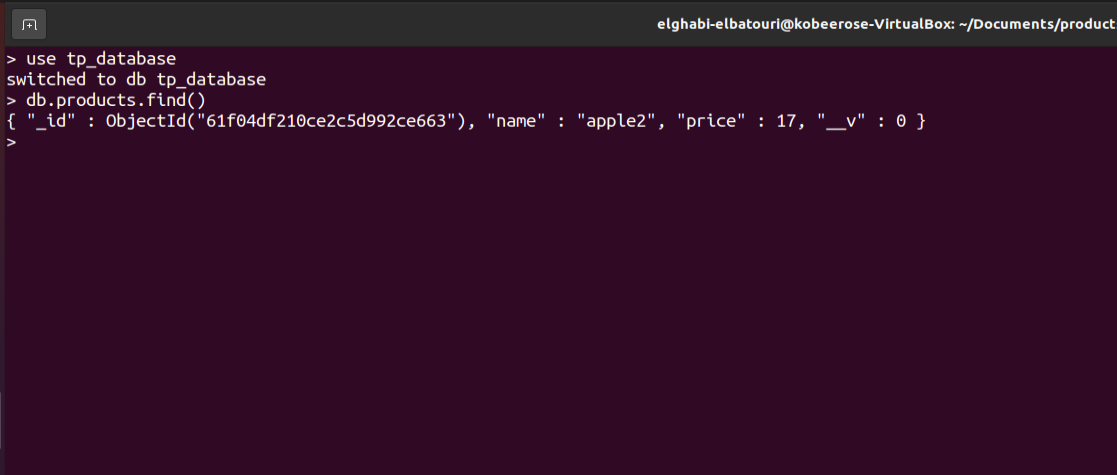
\includegraphics[width=1\linewidth]{Pictures/MongoDB/Nodejs and MongoDB CRUD  application/Implementing Endpoints/Verifying Changes in MongoDB} 
\end{center} 
\caption{Verifying Changes in MongoDB} 
\end{figure}  \FloatBarrier
\\

\newpage
\par The last task of our CRUD app is to delete an existing product.
To configure the route then we create the product\_update controller.
\begin{figure}[!htb] 
\begin{center} 
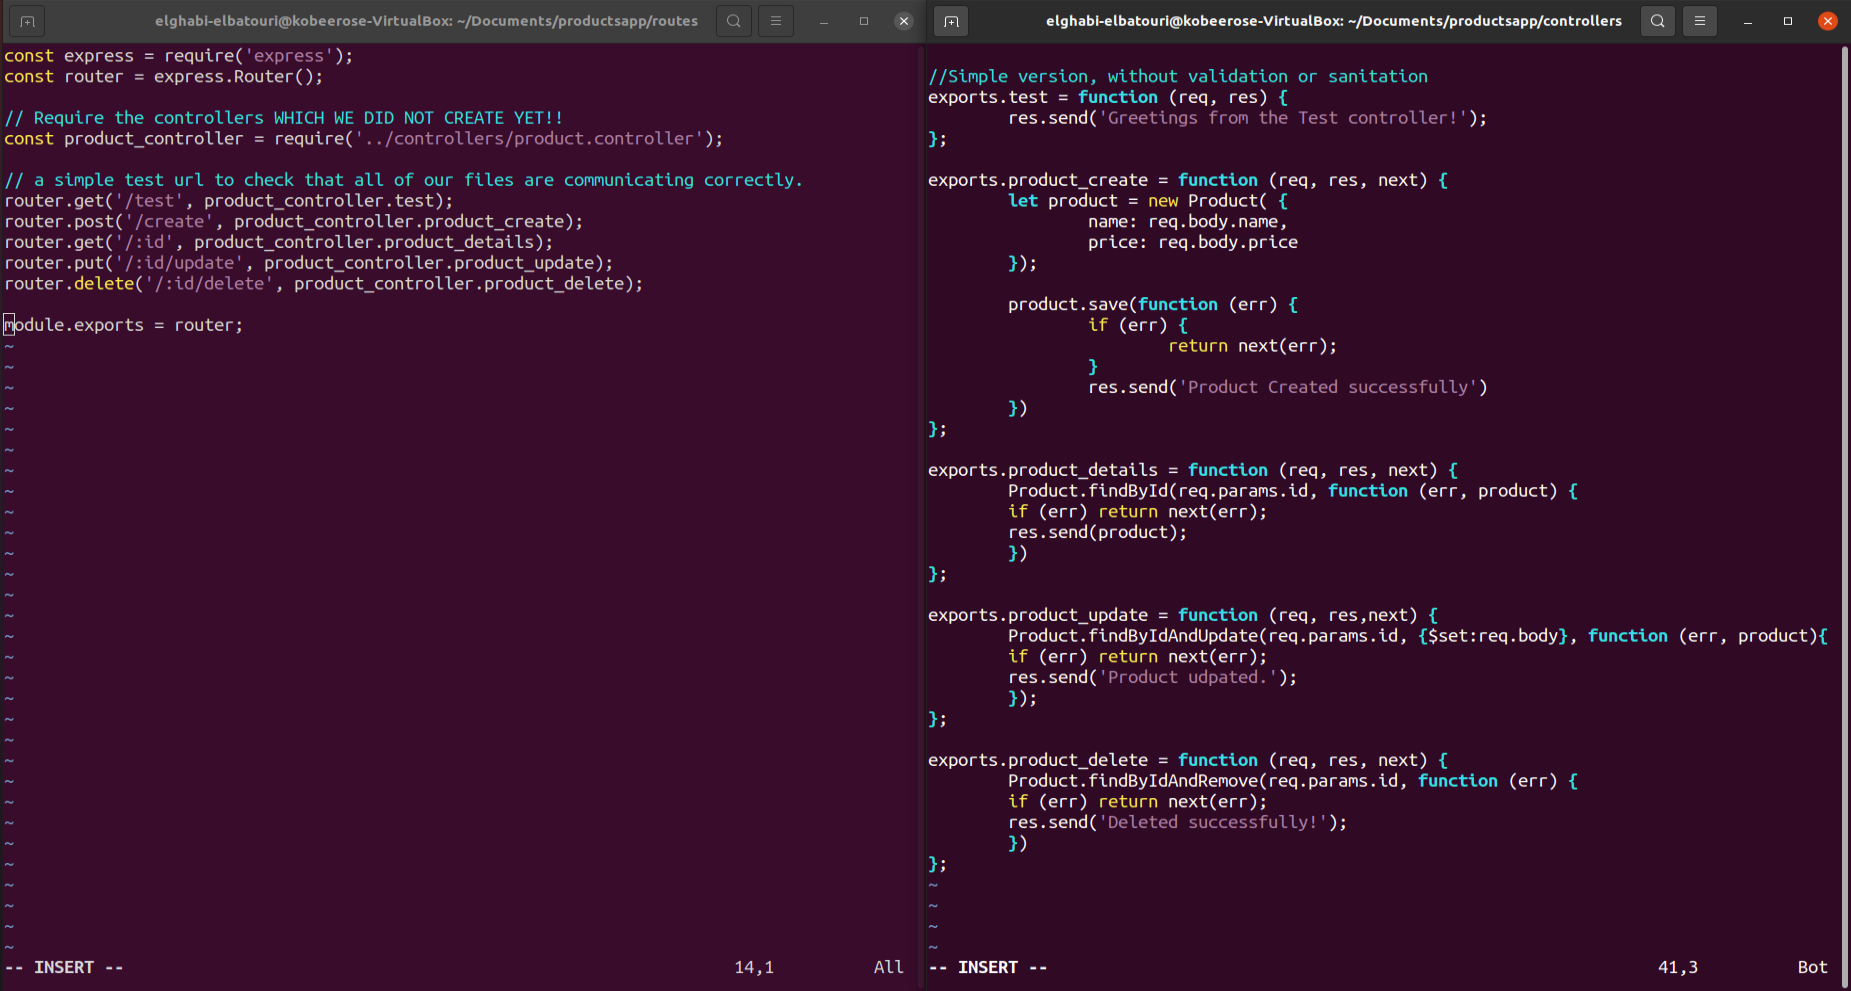
\includegraphics[width=1\linewidth]{Pictures/MongoDB/Nodejs and MongoDB CRUD  application/Implementing Endpoints/Router and Controller for DELETE} 
\end{center} 
\caption{Router and Controller for DELETE} 
\end{figure}  \FloatBarrier
\\

\par Choose "DELETE" and call the URL
following : “localhost:1234/products/PRODUCT\_ID/delete” PRODUCT\_ID is the ID of the object we created in the previous endpoint.
\begin{figure}[!htb] 
\begin{center} 
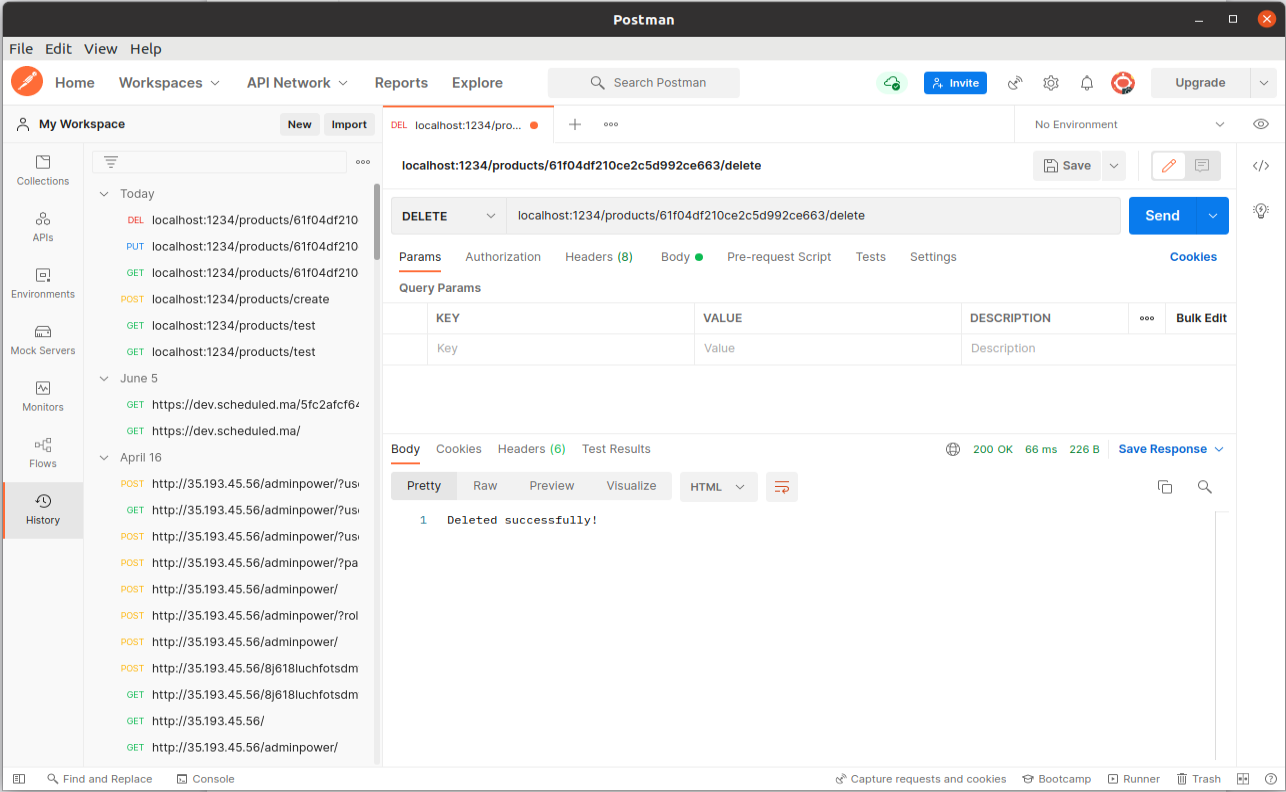
\includegraphics[width=1\linewidth]{Pictures/MongoDB/Nodejs and MongoDB CRUD  application/Implementing Endpoints/Testing DELETE endpoint} 
\end{center} 
\caption{Testing DELETE endpoint} 
\end{figure}  \FloatBarrier
\\
\newpage
\par To test these changes, we log in to Mongo's terminal and verify that the collection
products has been deleted.
\\
\begin{figure}[!htb] 
\begin{center} 
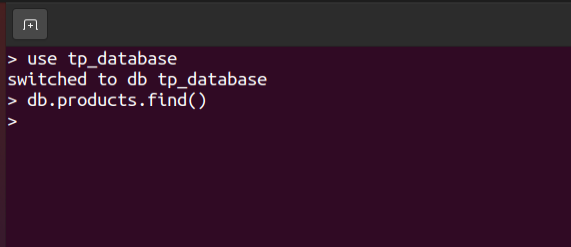
\includegraphics[width=1\linewidth]{Pictures/MongoDB/Nodejs and MongoDB CRUD  application/Implementing Endpoints/Empty db in mongo} 
\end{center} 
\caption{Empty db in mongo} 
\end{figure}  \FloatBarrier
\\

\end{spacing}